% Create by Assoc. Prof. Dr. Mohd Bakri bin Adam on 1 July 2016 to suit the B5 format for final submission for final binding with the help of Aisha the master student from Engineering Faculty%
% I recommended all users of this template to use TeXworks as the editor to get the best result with minimal adjustment %
% All users that need help please do not hesitate to email bakri@upm.edu.my%
% Additional materials are: inside the formats
% ---------------------------------------------------------------------------------------% 
% End result or printing will be depend on the printer that you're using This is depend on your printer 8 August 2016
\documentclass[b5paper,twoside,tocchapterhead,10pt]{UPMthesisEnglish}
%\documentclass[b5paper,twoside,openright,tocchapterhead,10pt]{UPMthesisEnglish}
\usepackage{wordlike}
\usepackage{hanging}
\usepackage{paralist}
\usepackage{afterpage}
\usepackage{natbib}
\usepackage[figuresright]{rotating}
\usepackage{lscape}
\usepackage{graphicx}
\usepackage{longtable}
\usepackage{calc}
\usepackage{amsmath}
\usepackage{amsfonts}
\usepackage{amssymb}
\usepackage{setspace}
\usepackage{color}
\usepackage{mdwlist}
\usepackage{wrapfig}
\usepackage{subfigure}
\usepackage{titlesec}
\usepackage[english]{babel}
\usepackage{mathrsfs}
\usepackage{bbding}
\usepackage{lipsum}
\usepackage{geometry}
\usepackage{lipsum}
\usepackage{bm}
\usepackage{bbold}
\usepackage{natbib}
\usepackage{enumerate}
\usepackage{enumitem}
\usepackage[figuresright]{rotating}
\usepackage{adjustbox}
\usepackage{tikz}
\usetikzlibrary{arrows,positioning,shapes.geometric}
\usepackage[font=bf]{caption}
\usepackage{paralist}
\usepackage{afterpage}
\usepackage{fancybox}
\usepackage{array}
\usepackage{algorithmicx}
\usepackage[caption=false]{subfig} %untuk caption multiple gambar dalam satu Figure)
\usepackage[chapter]{algorithm}
\usepackage{amsfonts}
\usepackage{algpseudocode}
\usepackage{float}
\usepackage{placeins}
\usepackage{epstopdf}
\usepackage{epsfig}
\usepackage{textcomp} 
\usepackage{pdflscape}
\usepackage{booktabs} %untuk cantikkan top & bottom horizontal line dalam table
\usepackage{multirow} %untuk split cell dalam table
\usepackage{url} % untuk support URL dalam \bibliographystyle{aisha} )
\usepackage{tipa} % aisha tambah 1/11/2011 (untuk special character dalam nama author dalam bibliografi)
\usepackage{array} % aisha tambah 20/11/2011 (untuk control table width dalam Appendix E)
%\usepackage[utf8]{inputenc}

\usepackage{makeidx}  % To create indices for the thesis
\graphicspath{ {images/} }
\usepackage{float}


\makeindex 



%\citestyle{ap6} % aisha ubah
%\usepackage[left=25mm,right=33mm,top=1in,bottom=1in]{geometry} %userpackage yg nih untuk set printout abstrak sehingga list of abbrev + next palin page - set 1
%\newcommand{\l}[1]{_{\!\mathsmaller{#1}}}
%\usepackage[left=33mm,right=25mm,top=1in,bottom=1in]{geometry} %userpackage yg nih untuk set printout pagetitle dan chapters - set 2
\newcolumntype{L}[1]{>{\raggedright\let\newline\\\arraybackslash\hspace{0.25pt}}m{#1}}
\newcolumntype{C}[1]{>{\centering\let\newline\\\arraybackslash\hspace{0.0cm}}m{#1}}
\newcolumntype{R}[1]{>{\raggedleft\let\newline\\\arraybackslash\hspace{0pt}}m{#1}}




% % % % % % % % % % % % % % % % % % % % % % % % % % % % % % % % % % % %


\titleformat{\section}
  {\normalfont\fontsize{10}{15}\rmfamily\bfseries}
  {\thesection}
  {1em}
  {}

\titleformat{\subsection}
  {\normalfont\fontsize{10}{15} \rmfamily\bfseries}
  {\thesubsection}
  {1em}
  {}
  
\titleformat{\subsubsection}
  {\normalfont\fontsize{10}{15}\rmfamily\bfseries}
  {\thesubsubsection}
  {1em}
  {}


\makeatletter
\renewcommand{\l@section}{\@dottedtocline{1}{1.5em}{2.6em}}
\renewcommand{\l@subsection}{\@dottedtocline{2}{4.0em}{3.6em}}
\renewcommand{\l@subsubsection}{\@dottedtocline{3}{7.4em}{4.5em}}
\makeatother




\addto\captionsenglish{%
 % \renewcommand{\figurename}{Fig.}%
  \renewcommand{\contentsname}{\bf Table of Contents}%
}
 
\setlength{\parskip}{10pt} % To make a blank line between two paragraphs


\newtheorem{thm}{Theorem}[section]
\newtheorem{lem}[thm]{Lemma}
\newtheorem{cor}[thm]{Corollary}
\newtheorem{prop}[thm]{Proposition}
\newtheorem{defin}[thm]{Definition}
\newtheorem{rem}[thm]{Remark}
\newtheorem{prob}[thm]{Problem}

\newtheorem{Theorem}{\quad Theorem}[section]

\newtheorem{Definition}[Theorem]{\quad Definition}

\newtheorem{Corollary}[Theorem]{\quad Corollary}

\newtheorem{Lemma}[Theorem]{\quad Lemma}

\newtheorem{Example}[Theorem]{\quad Example}





%\usepackage{atbegshi}% http://ctan.org/pkg/atbegshi
%\AtBeginDocument{\AtBeginShipoutNext{\AtBeginShipoutDiscard}} % Add on 3 May 2016 to remove first empty pages
\def \addblankpage{
\afterpage{
	\thispagestyle{empty}
	\newpage
	\mbox{}
	\newpage
	}
}

\begin{document}

\def \authorname{Demudu Naganaidu} %NAME OF STUDENT IN CAPITAL LETTERS
\def \authormatric{GS49320}
\def \thesistitle{Exploring Data with Histogram}% ENGLISH TITLE OF THESIS IN CAPITAL LETTERS
\def \thesistitleM{Eksplorasi Data dengan Histogram}% Malay TITLE OF THESIS IN CAPITAL LETTERS 3 May 2016
%\def \degree{Doctor of Philosophy} 
\def \degree{Doctor of Philosophy} % or Master of Science
\def \chair{Associate Professor Dr.  Mohd Bakri Bin Adam, Ph.D.}
\def \chairM{Professor Madya Dr.  Mohd Bakri Bin Adam, Ph.D.} % Malay
\def \memberA{Associate  Professor Dr. Jayanthi a/p Arasan, Ph.D.}
\def \memberB{Dr. Iskandar Bin Ishak, Ph.D.}
%\def \memberC{name of Member of Supervisory 3}
\def \chairViva{Professor Dr. E, Ph.D.}
\def \examinerA{Professor Dr. F, Ph.D.}
\def \examinerB{Associate Professor Dr. G, Ph.D.}
\def \examinerC{Dr. H, Ph.D.}
\def \thesisDate{August 2020}
\def \thesisDateM{Ogos 2020}
{
%\newgeometry{left=33mm,right=25mm,top=25mm,bottom=25mm}
\newgeometry{left=27mm,right=18mm,top=19mm,bottom=15mm} % Change 3 May 2016 Bakri This is depend on your printer 8 August 2016
\begin{titlepage}
\begin{center}
%\newpage
%\thispagestyle{empty}
\afterpage{\thispagestyle{empty}}

\includegraphics[angle=0,width=6.5cm,height=3.0cm]{upm.jpeg}

\vspace{15mm}%

\begin{singlespace}
	{\normalsize \bf {\textsc{\thesistitle}}}
	
	\vspace*{40mm}
	
	\bf {\textbf{\normalsize By}}

	\vspace{5mm}

	{\normalsize \bf{\textbf{\textsc{\authorname}}}} 


\vfill

	%\vspace*{45mm}
	
	
	{\normalsize \bf Thesis Submitted to the School of Graduate Studies, Universiti Putra Malaysia, in Fulfilment of the Requirements for the Degree of Doctor of Philosophy}
\end{singlespace}

\vspace{5mm}

{\normalsize \bf August 2020}
% Month and year of Viva Voce
\end{center}
\end{titlepage}
}

{
%\newgeometry{left=33mm,right=25mm,top=25mm,bottom=25mm}
\newgeometry{left=27mm,right=18mm,top=19mm,bottom=15mm} % Change 3 May 2016 Bakri This is depend on your printer 8 August 2016
\singlespacing
\begin{center}
{\normalsize \bf COPYRIGHT}
\end{center}
All material contained within the thesis, including without limitation text, logos, icons, photographs and all other artwork, is copyright material of Universiti Putra Malaysia unless otherwise stated. Use may be made of any material contained within the thesis for non-commercial purposes from the copyright holder. Commercial use of material may only be made with the express, prior, written permission of Universiti Putra Malaysia.\\\\
Copyright \textcopyright Universiti Putra Malaysia}


%----------------------------------------------------------------------------------------%
%----------------------------------------------------------------------------------------%
{
%\newgeometry{left=33mm,right=25mm,top=25mm,bottom=25mm}
\newgeometry{left=27mm,right=18mm,top=19mm,bottom=15mm} % Change 2 May 2016 This is depend on your printer 8 August 2016
%{\newgeometry{left=25mm,right=33mm,top=1in,bottom=1in}

{\singlespace \begin{center}
{\normalsize \bf DEDICATIONS}
\end{center}

\thispagestyle{empty}
\vspace{2cm}
\begin{center}

\it{To all of my love;\\
	Shinu \& Puran\\
	Mother \& Brothers and Sisters\\ 

	
}
\end{center}
}

	\newpage
	\thispagestyle{empty}
	\mbox{}
	\newpage


\pagenumbering{roman}
{
%\newgeometry{left=25mm,right=33mm,top=25mm,bottom=25mm}
\newgeometry{left=27mm,right=18mm,top=19mm,bottom=15mm} % Change 3 May 2016 This is depend on your printer 8 August 2016
% \newgeometry{left=33mm,right=25mm,top=1in,bottom=1in}
\addcontentsline{toc}{chapter}{\textbf{ABSTRACT}}
 \begin{singlespace}
\begin{center}
Abstract of thesis presented to the Senate of Universiti Putra
Malaysia in fulfilment of the requirement for the degree of Doctor of Philosophy

\vspace{5mm}%

{\normalsize \bf {\textsc{\thesistitle}}}
%\textsc{\bf \thesistitle}

\vspace{5mm}%

{\textsc By}

\vspace{5mm}%

{\bf {\textsc{\authorname}}}

\vspace{5mm}%

{\bf \thesisDate}

\end{center}

\vspace{5mm}


\begin{flushleft}
\begin{tabular}{ll}
Chairman &: {\bf  \chair}\\
Faculty &: {\bf Institute For Mathematical Research}
\end{tabular}
\end{flushleft}

\end{singlespace}
\vspace{5mm} %\doublespace 


Histogram is bla bla bla...
	
}

\addblankpage % disable this command if your abstract ONLY one page



{
%\newgeometry{left=33mm,right=25mm,top=1in,bottom=1in}
\newgeometry{left=27mm,right=18mm,top=19mm,bottom=15mm} % Change 3 May 2016 This is depend on your printer 8 August 2016
\addcontentsline{toc}{chapter}{\it \textbf{ABSTRAK}}
 \begin{singlespace}
\begin{center}
Abstrak tesis yang dikemukakan kepada Senat Universiti Putra
Malaysia sebagai memenuhi keperluan untuk ijazah Doktor Falsafah

\vspace{5mm}

\textsc {\bf \textsc  \thesistitleM}

\vspace{5mm}

{\textsc Oleh}

\vspace{5mm}

{\bf \textsc \authorname}

\vspace{5mm}

{\bf \thesisDateM}

\end{center}

\vspace{5mm}


\begin{flushleft}
\begin{tabular}{ll}
Pengerusi &: {\bf  \chairM}\\
Fakulti &: {\bf Institut Penyelidikan Matematik}
\end{tabular}
\end{flushleft}
\end{singlespace}
\vspace{5mm}

%\doublespace

	Histogram is bla bla bla...
	
}

\addblankpage % disable this command if your abstract ONLY one page



%----------------------------------------------------------------------------------------%
{
%\newgeometry{left=33mm,right=25mm,top=1in,bottom=1in} 
\newgeometry{left=27mm,right=18mm,top=19mm,bottom=15mm} % Change 3 May 2016 Bakri This is depend on your printer 8 August 2016
\addcontentsline{toc}{chapter}{\textbf{ACKNOWLEDGMENTS}}
\begin{center}
		{\bf ACKNOWLEDGEMENTS}
\end{center}
	\begin{singlespace}

		Histogram is bla bla bla...
		
		
		
		
		
		
	\end{singlespace}}
	
	
	
	
	
	
	
	
	
}



%----------------------------------------------------------------------------------------%
{
%\newgeometry{left=33mm,right=25mm,top=1in,bottom=1in} 
\newgeometry{left=27mm,right=18mm,top=19mm,bottom=15mm} % Change 3 May 2016 Bakri This is depend on your printer 8 August 2016
\addcontentsline{toc}{chapter}{\textbf{APPROVAL}}
% ----------------- Approval Sheet 1: Examination Committee ----------------%
\begin{center}
		{\bf THESIS EXAMINATION COMMITTEE}
\end{center}
	
	
\begin{singlespace}
I certify that a Thesis Examination Committee has met on
{{XX August 2020}} to conduct the final
examination of {{\authorname}} on his
thesis entitled "{{\thesistitle}}" in accordance with the
Universities and University Colleges Act 1971 and the Constitution
of the Universiti Putra Malaysia [P.U.(A) 106] 15 March 1998. The
Committee recommends that the student be awarded the {\degree}.

Members of the Thesis Examination Committee were as follows:

{\bf{\chairViva}}\\
Associate Professor\\
Faculty of Science\\
Universiti Putra Malaysia\\
(Chairperson)\\

{\bf{\examinerA}}\\
Associate Professor\\
Faculty of Science\\
Universiti Putra Malaysia\\
(Internal Examiner)\\

{\bf{\examinerB}}\\
Professor\\
School of Mathematical Sciences\\
Universiti Sains Malaysia\\
(External Examiner)\\

{\bf{\examinerC}}\\
Professor\\
Laboratoire de Math\'{e}matiques Nicolas Oresme\\
Universit\'{e} de Caen Basse Normandie\\
France\\
(External Examiner)\\\

\vfill

\begin{table}[b!]
\begin{tabular}{ll}
\hspace{7cm} &                                    \\
\cline{2-2} \vspace{-.3cm}                        \\
             & {\bf{ZULKARNAIN ZAINAL, Ph.D.}}\\
             & Professor and Deputy Dean          \\
             & School of Graduate Studies         \\
             & Universiti Putra Malaysia          \\
             &                                    \\
             & Date:           \\
\end{tabular}
\end{table}

\newpage



%\mbox{}
%%\newpage
% ---------------- Approval Sheet 2: Supervisory Committee ---------------- %
%\newpage
\begin{center}
		{\bf SUPERVISORY COMMITTEE}
\end{center}
	
This thesis was submitted to the Senate of Universiti Putra
Malaysia and has been accepted as fulfilment of the requirement
for the degree of {{\degree}}.

The members of the Supervisory Committee were as follows:

{\bf{\chair }}\\
Associate Professor\\
Faculty of Science\\
Universiti Putra Malaysia\\
(Chairperson)\\

{\bf \memberA}\\
Associate Professor\\
Faculty of Science \\
Universiti Putra Malaysia\\
(Member)\\

{\bf \memberB}\\
Senior Lecturer\\
Faculty of Computer Science and Information Technology\\
Universiti Putra Malaysia\\
(Member)\\

%{\bf \memberC}\\
%Senior Lecturer\\
%Kulliyyah of Engineering\\
%International Islamic Universiti Malaysia\\
%(Member)\\


%(Add or delete if there are more or less than three members in the supervisory committee, respectively)

\vfill

\begin{table}[b!]
\begin{tabular}{ll}
\hspace{5.5cm} &                            \\
\cline{2-2}  \vspace{-.3cm}               \\
             & {\bf BUJANG KIM HUAT, Ph.D.}   \\
             & Professor and Dean         \\
             & School of Graduate Studies \\
             & Universiti Putra Malaysia  \\
             &                            \\
             & Date:                     \\
\end{tabular}
\end{table}
\end{singlespace}

%\newpage

%\mbox{}


}


%----------------------------------------------------------------------------------------%
%----------------------------------------------------------------------------------------%

{
%\newgeometry{left=33mm,right=25mm,top=1in,bottom=1in} 
\newgeometry{left=27mm,right=18mm,top=19mm,bottom=15mm} % Change 3 May 2016 Bakri This is depend on your printer 8 August 2016
%\begin{center}
%{\normalsize \textbf{DECLARATION}}
%\end{center}
%\vspace{7mm}

\begin{center}
		{\bf STUDENT DECLARATION}
\end{center}

\noindent {\bf Declaration by graduate student}

%\vspace{0.2cm}

\noindent I hereby confirm that:
\begin{itemize}[label={$\bullet$},noitemsep,leftmargin=*,topsep=0pt,partopsep=0pt]
\vspace{-10pt} 
		\item this thesis is my original work;
		\item quotations, illustrations and citations have been duly referenced;
		\item this thesis has not been submitted previously or concurrently for any other degree at any other institutions;
		\item intellectual property from the thesis and copyright of thesis are fully-owned by Universiti Putra Malaysia, as according to the Universiti Putra Malaysia (Research) Rules 2012;
		\item written permission must be obtained from supervisor and the office of Deputy Vice-Chancellor (Research and Innovation) before thesis is published (in the form of written, printed or in electronic form) including books, journals, modules, proceedings, popular writings, seminar papers, manuscripts, posters, reports, lecture notes, learning modules or any other materials as stated in the Universiti Putra Malaysia (Research) Rules 2012;
		\item there is no plagiarism or data falsification/fabrication in the thesis, and scholarly integrity is upheld as according to the Universiti Putra Malaysia (Graduate Studies) Rules 2003 (Revision 2012-2013) and the Universiti Putra Malaysia (Research) Rules 2012. The thesis has undergone plagiarism detection software.
	\end{itemize}


\vspace{0.2cm}

\noindent Signature:\hrulefill  Date:\hrulefill

\vspace{0.5cm}

\noindent Name and Matric No: \underline{ \authorname, \authormatric}

\newpage

%\mbox{}

%\newpage

\begin{center}
		{\bf SUPERVISORY COMMITTEE DECLARATION}
\end{center}

\noindent {\bf Declaration by Members of Supervisory Committee}

\vspace{0.2cm}
This is to confirm that:
\begin{itemize}[label={$\bullet$},noitemsep,leftmargin=*,topsep=0pt,partopsep=0pt]
	\vspace{-10pt} 
\item the research conducted and the writing of this thesis was under our supervision;
\item supervision responsibilities as stated in the Universiti Putra Malaysia (Graduate Studies) Rules 2003 (Revision 2012-2013) are adhered to.
\end{itemize}

\vspace{1cm}
Signature: \line(1,0){150} \\
Name of 
Chairman of
Supervisory 
Committee\\ {\bf \chair}\\ 
%(Chairperson)\\

\vspace{1cm}
Signature: \line(1,0){150} \\
Name of 
Member of
Supervisory
Committee \\ {\bf \memberA}\\
%(Member)\\

\vspace{1cm}
Signature: \line(1,0){150} \\
Name of 
Member of
Supervisory
Committee\\ {\bf \memberB}\\
%(Member)\\




%\if 0
%\begin{tabular}{cc}
%\begin{tabular}{c}
%Signature: \\
%Chairman
%\end{tabular} &
%\begin{tabular}{c}
%Signature: \\
%Member
%\end{tabular} \\
%\begin{tabular}{c}
%Signature: \\
%Member 
%\end{tabular} &
%\end{tabular}
%\fi 



}


%\newpage

%----------------------------------------------------------------------------------------%
%--- The following command is to remove the dots from the list of the tables, figures ---%
%--- and the table of contents                                                        ---%
\makeatletter \renewcommand{\@dotsep}{10000} \makeatother
%----------------------------------------------------------------------------------------%

\addblankpage % disable this command if your TABLE OF CONTENTS STARTED ON YOUR RIGHT HAND SIDE PAGE or ODD PAGE NUMBER 

\newgeometry{left=27mm,right=18mm,top=19mm,bottom=15mm} % Change 3 May 2016 This is depend on your printer 8 August 2016

\tableofcontents

\addblankpage % disable this command if your LIST OF TABLES STARTED AT EVEN PAGE NO.

\listoftables

\addblankpage % disable this command if your LIST OF FIGURES  STARTED AT EVEN PAGE NO.

\listoffigures

\addblankpage % disable this command if your LIST OF ABBREAVIATONS STARTED EVEN PAGE NO

\addcontentsline{toc}{chapter}{\textbf{LIST OF ABBREVIATIONS}}

\begin{center}
\normalsize{\textbf{LIST OF ABBREVIATIONS}} \vspace{1cm}
\end{center}

%%%%%%%%%%%%%%%%%%%%%%%%%%%%%%%%%%%%%%%%%%%%%%%%%%%%%%%%%%%%%%%%%%%%%
% If abbreviations and acronyms (e.g. MARDI, UPM) are used in the   %
% thesis, they should be explained in a List of Abbreviations, even %
% though the full names are given when the terms are first          %
% mentioned in the text. This list should be the last item in the   %
% preliminary section. It serves as a ready reference to readers    %
% not familiar with the abbreviations used in the thesis.           %
% Universally recognised scientific symbols (such as cm, mm, kg)    %
% need not be listed.                                               %
%%%%%%%%%%%%%%%%%%%%%%%%%%%%%%%%%%%%%%%%%%%%%%%%%%%%%%%%%%%%%%%%%%%%%

\begin{center}
\begin{tabular}{ll}
BFHP 		&\hspace{2cm} Bivariate Function Hard Problem \\
CCA			&\hspace{2cm} Chosen Ciphertext Attack\\
CCA1		&\hspace{2cm} Non-adaptive CCA\\
CCA2		&\hspace{2cm} Adaptive CCA\\
CPA			&\hspace{2cm} Chosen Plaintext Attack\\
CRT    		&\hspace{2cm} Chinese Remainder Theorem \\
$\gcd$		&\hspace{2cm} Greatest Common Divisor \\
IFP			&\hspace{2cm} Integer Factorization Problem \\
IND			&\hspace{2cm} Indistinguishability\\
IND-CCA2	&\hspace{2cm} Indistinguishable against CCA2\\
LLL			&\hspace{2cm} Lenstra-Lenstra-Lovasz\\
OAEP		&\hspace{2cm} Optimal Asymmetric Encryption Padding\\
ROM			&\hspace{2cm} Random Oracle Model\\
RSA			&\hspace{2cm} Rivest-Shamir-Adleman\\
SET			&\hspace{2cm} Secure Electronic Transaction \\
$spm$		&\hspace{2cm} Single-precision Multiplication \\
\end{tabular}
\end{center}









\addblankpage

%\addblankpage % disable this command if your abstract ONLY one page



%----------------------------------------------------------------------------------------%
\mainmatter
%\doublespace
\singlespace
\newgeometry{left=27mm,right=18mm,top=19mm,bottom=15mm} % Change 3 May 2016 This is depend on your printer 8 August 2016
%----------------------------------------------------------------------------------------%
% The Command:                                                                           %
% \addtocontents{toc}{\addvspace{.5cm}}                                                  %
% must be added before each \include {chapter}                                           %
%----------------------------------------------------------------------------------------%

\addtocontents{toc}{\addvspace{.5cm}}
\chapter{\textbf{INTRODUCTION}}\label{Introchap} 
%\chapter{\normalsize \textbf{CHAPTER 1}}} \label{Introchap}

\section{Background}

We see technology advancement as continuous phenomena: new applications and devices introduced every now and then such as social media, Internet banking, E-Commerce, Massive Open Online Courses (MOOC) , Smartphone's, TAB's, IPAD's, Wearable Sensors, Self-Driving Car and etc. These new applications and devices which are important aspect of our daily activities, creates massive data \cite[]{torrecilla2018data}. Learning from these data is important for decision making and to improve the process and productivity. 

However raw data are often large, making learning from these are almost impossible. Data must be organized, summarized and described in the form that facilitate us to gain information and knowledge. Statistics is a science of collecting and transforming data into useful information for understanding and making informed decisions. Descriptive statistics which is one of the major two branches of statistic is commonly used to explore the data before any statistical test performed known as inferential statistics. 

Exploratory Data Analysis (EDA) is one of the method used in descriptive statistics. EDA was introduced by John W. Tukey in 1977 \cite[]{wendy2002computational}. EDA is mostly involves statistical graphs, is an approach of analyzing data visually without a prior assumptions on parametric model of the data, error terms, outliers in data, modality of the data and relationship with other variables \cite[]{velleman1981applications,wendy2002computational}. Visualising data is vital in exploring data \cite[]{scott2005multidimensional} to help in finding the  patterns, structure in data and relationships between variables in data \cite[]{hand2001principles}. EDA helps the researchers to model data based on the what is revealed through exploring with various graphical methods. Generally after the EDA process one would use confirmatory analysis such as hypothesis testing, ANOVA, regression and etc.

Histogram is one of the important tools used in EDA. It is used often in graphical analysis to visualise data \cite[]{li2016essential}. The subject of histogram is so important that it is included in every elementary statistics or data analysis course. 

\section{Histogram}

Histogram useful in summarising large amount numerical data graphically \cite[]{kirschenmann2015note} and to visualise the distribution of data without prior assumptions on the characteristics of data or the underlying true distribution of the data. Hence histogram is called as a non-parametric density estimator\cite[]{keen2010graphics}. Once a histogram is constructed the general attributes of the data such as symmetry, modality, central location and spread of the data will be revealed.

A typical histogram is a stack of rectangular columns each of whose heights is proportional to the corresponding frequency of data values. Data values grouped into intervals, called as bins (or classes). In constructing histogram number bins or equally the bin width must be decided upfront. Bins can be either same size (i.e equal width) or different size (i.e unequal width) provided it should encompass all the data and non overlap with each other. Number of bins used to construct histogram will determines the shape of it. Too many bin makes the histogram uneven and unable to find the underlying trend of the data. Too few bin gives little information about the data. 

\section{Histogram Bins}

Number of bins in grouping data can be predefined upfront or using some scientific rules. For example data on marks in a exam can be grouped into 5 bins: 0-20, 20 - 40, 40-60, 60-80 and 80-100. Alternatively one can use rules such Sturges(1926) rule as a guide to decide number of bins. For sample data of size 40, the Sturges(1926) rule suggest 7 bins. More discussion on rules in Chapter 2 - Literature Review.

%Most statistical packages default settings uses Sturges' rule in calculating number of bins. Herbert Sturges(1926) proposed a simple rule for classifying a series of n items. %The expectation is that a normally distributed variable can be appropriately divided so that the bin frequencies comprise a binomial series for all n which are powers of 2. 
%Doane (1976) provide a modification to Sturges' rule which attempts to improve its construction of histogram with skewed data. Beside Doane (1976), Scott's (1979) and Freedman and Diaconis's (1981) gives alternative rules for constructing histogram by the bin width. 


\section{Numerical Data }

Numerical data can be classified into discrete and continuous data. 

A set of data is said to be discrete if the values belonging to the data set only assumes integer values as 0,1,2,3,4 and etc. There are gaps between two possible values in a discrete dataset. Examples of discrete data are number of children in a family, number of cars on the road, number of students in a school, number of defective items and etc.

Continuous data assumes any values between two specific values. Continuous data are normally obtained by measuring. There are no gaps in between any two possible values in a continuous dataset. Examples of continuous data are height of students in an university, amount of rain in a month, volume of water (in ml) in a bottle, and etc. 

\section{Raw Data and Grouped Data}
 
Dataset can be presented as raw (ungrouped) or grouped data. Raw data is usually unsorted are given as list of data values in the dataset. Grouped data is the raw data that has been sorted into a set classes or intervals or bins. While discrete data can be summarised using a frequency table continuous data must grouped in a set of bins before the frequency table can produced.


\section{Frequency}

Frequency is simply counts of a data value appears in a given dataset.  Frequency of a dataset displayed using a table format known as frequency table based on the classes or bins. Obtaining  frequency of dataset is the first step in summarising dataset before producing graphical charts for visualisation.




\section{Frequency Table}




\section{Frequency Polygon}

\section{Bar Chart}

\section{Use of Histogram}

Histogram can provide a clue to researchers of a possible parametric model suitable for data  \cite[]{wendy2002computational} besides detecting unusual observations or behavior in data. Histogram can be used to estimate the 5 number summary of data and variation in data.

Histogram is widely used as one of the Seven (7) Quality Control Tools (7QC) to ensure manufacturing process are within the controlled specification or to maintain the quality level \cite[]{magar2014application}. 


Histogram based image processing that is very useful for medical image analysis, industrial X-ray and etc is used widely because easy to understand and implement besides being effective \cite[]{sharma2015review}.


Regression with Histogram Data.

\section{Problem Statement}

Deciding how many bins to be used is still a challenge to most researchers especially when background of the data is unknown. Despite there many suggested methods to determine the number of bins, there is no single method is agreed upon. The five number summary and variation calculated from raw data can used in deciding the number bins.

Detecting the outliers from histogram not very helpful due the method of constructing. The modification of construction histogram can reveal the outliers more effectively.


\section{Research Aims and Objectives}

This study aims to achieve following objectives:

\begin{itemize}
	\item propose a method using raw data five number summary and variation to decide the number of bins.
	\item evaluate new method with existing methods
	\item propose a new method for construction of histogram to detect outliers
	\item evaluate new method against box-plot method to detect outliers
	\item propose a fixed frequency histogram for the purpose of segmentation 

\end{itemize}



\section{Limitation of Study}

\section{Structure of Thesis}


\addblankpage % disable this if the last page for this chapter is even

\chapter{\textbf{LITERATURE REVIEW}}\label{Introchap} 
%\chapter{\normalsize \textbf{CHAPTER 1}}} \label{Introchap}

\section{History of Histogram}

The term "histogram" was introduced by Karl Pearson \cite[]{ross2010introductory, rufilanchas2017origin} but there was confusion on the date or year it was introduced \cite[]{rufilanchas2017origin,ioannidis2003history}. Several authors stated the year as 1895 \cite[]{beniger1976history, dodge2008concise,ross2010introductory,li2016essential}. However \cite[]{magnello2014introducing, rufilanchas2017origin} clarified that the histogram was first introduced in 1891 in Gresham Lectures. Karl Pearson used the term while lecturing on "Maps and Chartograms" \cite[]{rufilanchas2017origin}.

Beside confusion on year of the term "histogram" was introduced there is also some confusion on the meaning of "histogram". The term is frequently misunderstood that it is used to study history \cite[]{rufilanchas2017origin}.  The association of histogram as historical diagram was due to the fact that Karl Pearson use time histogram in his lecture to describe the "time-diagram" but he do not meant histogram used to study the subject "history" \cite[]{rufilanchas2017origin}.

Histogram has been used long before it received its name i.e from seventeen century. \cite[]{scott1979optimal,loquin2008histogram} believes that John Graunt (as cited in Westergard , 1968, p.22) probably was using histogram in 1662. John Graunt(1662) used a histogram to describe the mortality rate \cite[]{copas1983non,scott2005multidimensional}.  However \cite[]{chen2007handbook,ross2010introductory,rufilanchas2017origin} believes that William Playfair (1759- 1823) who invented bar chart was the person responsible in introducing histogram in 1801.  

Andre-Michael Guerry (A.M Guerry) a French mathematician was also given credit in introducing histogram in 1833 when he use William Playfair's bar chart concept on continuous data by categorizing i.e data on age and time. \cite[]{beniger1976history,friendly2007m,ross2010introductory}. A.M. Guerry produced his first publication in 1829 about crime in France population. In 1833 he return with his second publication by refining and extending data on his first published work. His third and major work that happened in 1864. Third publication used histogram as one of the main tool in presenting the comparison of crime against population between France and England \cite[]{friendly2007m}.

According to \cite[]{ross2010introductory} the systematic development in histogram was due to the work of Adolphe Quetelet in 1846 where he introduce methodological steps in doing research. Quetelet who was a Belgian statistician gave importance to graphical visualization for social science researches. Since then the histogram was further developed such as comparing data from different categories. For example Francis A. Walker[1840-1897] in producing the Atlas of Ninth Census for U.S nationals in 1874 incorporated a bilateral histogram to show graphically the distribution of deaths by sex and month of death and according to race and nationality \cite[]{beniger1976history, friendly2008golden}. 

Despite being one of the oldest graphical display tool, histogram is still being relevant for presenting univariate continuous data  visually \cite[]{scott1979optimal, wand1997data} and also being used in recent "Big Data Analytics" \cite[]{berger2016big}.

\addblankpage % disable this if the last page for this chapter is even

\chapter{\textbf{METHODOLOGY}}\label{Introchap} 
%\chapter{\normalsize \textbf{CHAPTER 1}}} \label{Introchap}

%\section{Variations on the Histogram}
%
%One of the histogram use: it's a nonparametric density estimator for an underlying true density function $f(x)$ \cite[]{waterman1978estimation,scott1979optimal} besides being useful for summarising and visualising data. We know from calculus that for any continuous variable $X$, the area under density function must be equal to one, a principle based on probability. 
%
%\begin{equation}
%\int_{- \infty}^{\infty} f(x) \, dx = 1 , f(x) \geq 0
%\end{equation}
%
%\begin{figure}[h]
%	\caption{Density Plot}
%	\centering 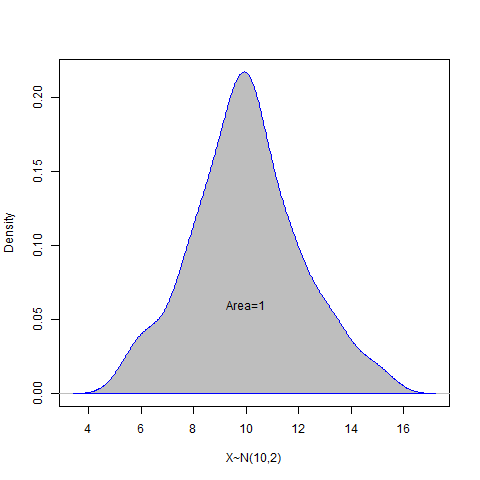
\includegraphics[scale=0.5]{density}
%\end{figure}
%
%Same principles applies to the histogram being empirical density estimator: the area under represented by histogram must be equal to one. 
%
%\begin{figure}[h]
%	\caption{Histogram with Density Plot}
%	\centering 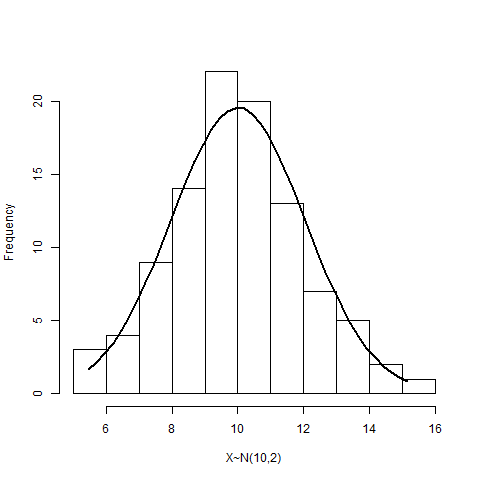
\includegraphics[scale=0.5]{hist_density}
%\end{figure}
%
%\clearpage
%
%As such any variation in histograms must satisfy this principles at all time. 

%\subsection{Equal width Histogram}


The most common histogram found and being used to explore the distribution of data. Each bin in equal width and non overlap.

\begin{figure}[h]
	\caption{Equal Width Histogram}
	\centering 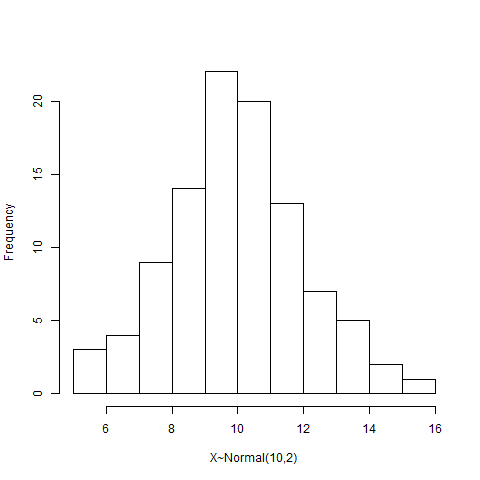
\includegraphics[scale=0.5]{hist_equalwidth}
\end{figure}

\section{Classical Histogram}

classical histogram testing

\subsection{Flow of Constructing Histogram}
\begin{enumerate}
	\item Selecting Bin Width
	\item Selecting Starting Point for First Bin
	\item Constructing the frequency Table
	\item Constructing the Histogram
\end{enumerate}

\begin{enumerate}
	\item Selecting Number of Bin
	\item Selecting Starting Point for First Bin
	\item Constructing the frequency Table
	\item Constructing the Histogram
\end{enumerate}
\subsection{Selection of Bins}

\subsection{Equal Width}

\subsection{Unequal Width}

\subsection{Symmetrical Data}

\subsection{Heavy Tail Data}
 
\subsection{Big Data and Small Data}
\subsection{Missing Data}
 

Frequency Table



compare the distribution with normal,

\section{Selecting the Best Histogram Representing Data}
\subsection{Goodness of Fit for Histogram}
\subsection{Statistics from frequency table}
\section{Modification of Constructing Histogram}

\subsection{Modification via Bin Numbers}

\subsection{Modification Via Bin Width}

\subsection{Modification for Heavy Tail Data}

\subsection{Starting point of constructing the histogram}

\section{Handling Big Data with Histogram}

\section{Histogram by Area}


\section{Modification  of Histogram} 
\subsection{Mode Formula}
\subsection{Mean Formula}
\subsection{Kurtosis}

\section{Histogram by Area\ Fall Down(Order Frequency Histogram)}

\section{Percentile Histogram}


\addblankpage % disable this if the last page for this chapter is even


%\addblankpage put this command at the last page of introduction.tex if your THE NEXT CHAPTER STARTED AT EVEN PAGE NUMBER 




%----------------------------Additional chapters may be added ---------------------------%
%                                                                                        %
%----------------------------------------------------------------------------------------%
% Bibliography on Chicago Thesis Style with modifications by Rand Alfaris.               %
% Don't make any changes on the following, except for the name of the bibliography file. %
% For example, we choose here a file named "bibli".                                      %
%----------------------------------------------------------------------------------------%
\addcontentsline{toc}{chapter}{\textbf{BIBLIOGRAPHY}}
\renewcommand\bibname{BIBLIOGRAPHY}
\begin{singlespace}
\bibliography{bibbliografi} % This is your bibtex file need to click BibTeX a few times alternate with pdfLaTeX
\bibliographystyle{apa6}
%\bibliographystyle{apj}
\end{singlespace}

%\begin{singlespace}
%\bibliography{bibli2013,bibli2013A,bibli2013B}
%\bibliographystyle{plainnat}
%\bibliographystyle{abbrvnat}
%\bibliographystyle{unsrtnat}
%\bibliographystyle{authordate1}
%\bibliographystyle{apalike}
%%\bibliographystyle{biometrika}
%\end{singlespace}
%----------------------------------------------------------------------------------------%


Learning from data is increasingly important in 21st century. We encounter data in our lives on daily basis mostly quantitative data such as prices of goods, weather, exam marks, sales, share prices , account balances, blood pressure reading, height, weight , body mass index and etc. Qualitative data can easily converted to quantitative data by coding.(Alternate Introduction)

Fortunately new fields of study such as Data Analyst, Data Science, Big Data and Data Analytic are also emerged for us to learn from these massive data.  

According to Chambers et al., " There is no single statistical tool that is as powerful as a well chosen graph". Often graphical summaries of data are very revealing and helpful in detecting outliers. One of the most commonly used and understood graphical summaries of values of numeric variables is the histogram. \cite{francis2005dancing}.

A histogram is useful to look at when we want to see more detail on the full distribution
of the data. The boxplot is quick and handy, but fundamentally only gives us a bit of
information. \cite{peng2012exploratory}

Why Graphics?
There is no single statistical tool that is as powerful as a well-chosen
graph. Our eye-brain system is the most sophisticated information
processor ever developed, and through graphical displays we can put
this system to good use to obtain deep insight into the structure of data.
An enormous amount of quantitative information can be conveyed by
graphs; our eye-brain system can summarize vast information qUickly
and extract salient features, but it is also capable of focusing on detail.
Even for small sets of data, there are many patterns and relationships
that are considerably easier to discern in graphical displays than by any
other data analytic method.\cite{john1983graphical}

A descriptive data analysis seeks to summarize the measurements
in a single data set without further interpretation \cite{leek2015elements}

An exploratory data analysis builds on a descriptive analysis
by searching for discoveries, trends, correlations, or relationships
between the measurements of multiple variables to
generate ideas or hypotheses. \cite{leek2015elements}

In a quality statistical data analysis the initial step has to be exploratory. This is
particularly true of applied data mining, which essentially consists of searching
for relationships in the data at hand, not known a priori.\cite{giudici2005applied}


More than 50 years ago, John Tukey called for a reformation of academic statistics. In `The
Future of Data Analysis', he pointed to the existence of an as-yet unrecognized science, whose
subject of interest was learning from data, or `data analysis'. Ten to twenty years ago, John
Chambers, Bill Cleveland and Leo Breiman independently once again urged academic statistics
to expand its boundaries beyond the classical domain of theoretical statistics; Chambers called
for more emphasis on data preparation and presentation rather than statistical modeling; and
Breiman called for emphasis on prediction rather than inference. Cleveland even suggested the
catchy name Data Science" for his envisioned field. \cite{donoho201750}


\addcontentsline{toc}{chapter}{\textbf{BIODATA OF STUDENT}}
\begin{center}
\normalsize{\textbf{BIODATA OF STUDENT}}
\end{center}


\thispagestyle{empty}


The student, \textbf{\authorname}, was born in May 1985. Obtained his bachelor degree in Mathematics Education from Universiti Teknologi Malaysia in 2008. He then received a Master of Sciences, from the Institute for Mathematical Research, Universiti Putra Malaysia in 2010. He is currently enrolled a doctoral study in the area of Mathematical Cryptography. He also acts as the secretary of the Malaysian Society of Cryptology Research (MSCR). His research interest involves with designing asymmetric cryptosystems, mathematical cryptanalysis and provable security. The student can be reached via email address; ma\_asyraf@upm.edu.my.


% email / phone / fax

%Or directly by email at gulaley@gmail.com.\\







\if %----------------------------------------------------------------------------------------%

This section is compulsory. It gives the student’s biographical information:
name, educational background, the degree that is being sought, professio-
nal work experience (if any), and any other similar matters that may
interest the reader. The vita should be in essay form, rather than a mere
résumé.



Nama
MyKad
Previous academic qualifications
Date registered for MSc
Duration of study
Sponsorship if any
Dept address for correspondence
E-mail
H/P



\fi % ---------------------------------------------------------------------------------------%   % Biodata of student                                                 %
\addcontentsline{toc}{chapter}{\textbf{LIST OF PUBLICATIONS}}
\begin{center}
\normalsize{\textbf{LIST OF PUBLICATIONS}}
\end{center}

% Only JOURNAL OR PROCEDING THAT HAS BEEN PUBLISHED SHOULD BE WRITTEN HERE. 
% PRESENTATION AT ANY CONFERENCE  OR SEMINAR SHOULD NOT BE WRITTEN HERE


The following are the list of publications that arise from this study.

Journal articles:


\begin{hangparas}{.25in}{1}
\textbf{Muhammad Asyraf Asbullah} and Muhammad Rezal Kamel Ariffin (2015). Design of Rabin-like Cryptosystem without Decryption Failure, \textit{Malaysian Journal of Mathematical Sciences} (Accepted for Publication).

\textbf{Muhammad Asyraf Asbullah} and Muhammad Rezal Kamel Ariffin (2015). Design of Rabin-like Cryptosystem without Decryption Failure, \textit{Malaysian Journal of Mathematical Sciences} (Accepted for Publication).

\end{hangparas}

	


Proceedings:

\begin{hangparas}{.25in}{1}
 \textbf{Muhammad Asyraf Asbullah} and Muhammad Rezal Kamel Ariffin (2012). A Proposed CCA-Secure Encryption on an ElGamal Variant. \textit{In the Proceeding of the $7^{th}$ International Conference on Computing and Convergence Technology 2012}, 3 - 5 December 2012, Seoul, pp. 499-503.
\end{hangparas}



\newpage
\thispagestyle{empty}
\cleardoublepage
 % List of publications                                      %
%\addcontentsline{toc}{chapter}{\textbf{STATUS CONFIRMATION FOR THESIS/PROJECT REPORT AND COPYRIGHT}}

%\backmatter 
\addcontentsline{toc}{chapter}{\textbf{INDEX}}
\printindex  % Need to click MakeIndex a few time same like BibTeX

\begin{titlepage}
\pagenumbering{gobble}
\small
\begin{center}

\includegraphics[angle=0,width=3.5cm]{upm.jpeg}
\end{center}

%\begin{doublespace} 
\begin{center}
{\bf \textbf{UNIVERSITI PUTRA MALAYSIA \\ STATUS CONFIRMATION FOR THESIS/PROJECT REPORT AND COPYRIGHT\\ACADEMIC SESSION:}} {\underline{2016/2017}}
\end{center}
%\end{doublespace}

{\bf \textbf{TITLE OF THE THESIS/PROJECT REPORT:}}\\
\underline{  {\textsc{\thesistitle}}          }



{\bf{NAME OF STUDENT:}} \underline{\authorname}
\begin{singlespace}
I acknowledge that the copyright and other intellectual property in the thesis/project report belonged to Universiti Putra Malaysia and I agree to allow this thesis/project report to be placed at the library under the following terms:

\begin{enumerate}
\item This thesis/project report is the property of Universiti Putra Malaysia.
\item The library of Universiti Putra Malaysia has the right to make copies for educational purposes only.
\item The library of Universiti Putra Malaysia is allowed to make copies of this thesis for academic exchange.
\end{enumerate}

I declare that this thesis is classified as:

*Please tick(\checkmark)
% amssymb
%\checkmark

% bbding
%\Checkmark
%\CheckmarkBold

% pifont
%ding{51}
%\ding{52}

% wasysym
%\CheckedBox
\begin{tabular}{lll}
\setlength\fboxsep{6pt}\cornersize*{7mm} \Ovalbox{\qquad} & CONFIDENTIAL & (contain confidential information under Official Secret \\ & & Act 1972).\\
\setlength\fboxsep{6pt}\cornersize*{7mm} \Ovalbox{\qquad} & RESTRICTED & (Contains restricted information as specified by the \\ 
& & organization/institution where research was done).\\
\setlength\fboxsep{6pt}\cornersize*{7mm} \Ovalbox{\qquad} & OPEN ACCESS & I agree that my thesis/project report to be published \\ & & as hard copy or 
online open acces.\\
%\end{tabular}
\multicolumn{2}{l}{This thesis is submitted for:} &\\
%\begin{tabular}{cll}
\setlength\fboxsep{6pt}\cornersize*{7mm} \Ovalbox{\qquad} & PATENT & Embargo from \line(1,0){50} until \line(1,0){50}.\\
& & \qquad \qquad \qquad \quad (date) \qquad \qquad \quad (date)\\
& & {\bf Approved by:}\\
& & \\
\line(1,0){70} && \line(1,0){70}\\
\multicolumn{2}{l}{(Signature of Student)} & (Signature of Chairman of Supervisory Committee)\\
\multicolumn{2}{l}{New IC No/Passport No.:850523-10-5567}& Name: {\bf \chair} \\
& &\\
Date: & & Date:\\
\end{tabular}

\vfill

{\bf[Note: If the thesis is CONFIDENTIAL or RESTRICTED, please attach with the letter from the organization/institution with period and reasons for confidentially or restricted.]}
\end{singlespace}

\end{titlepage}

 % Status confirmation for the thesis



\end{document}
%----------------------------------------------------------------------------------------%
